% Options for packages loaded elsewhere
\PassOptionsToPackage{unicode}{hyperref}
\PassOptionsToPackage{hyphens}{url}
%
\documentclass[
  ignorenonframetext,
]{beamer}
\usepackage{pgfpages}
\setbeamertemplate{caption}[numbered]
\setbeamertemplate{caption label separator}{: }
\setbeamercolor{caption name}{fg=normal text.fg}
\beamertemplatenavigationsymbolsempty
% Prevent slide breaks in the middle of a paragraph
\widowpenalties 1 10000
\raggedbottom
\setbeamertemplate{part page}{
  \centering
  \begin{beamercolorbox}[sep=16pt,center]{part title}
    \usebeamerfont{part title}\insertpart\par
  \end{beamercolorbox}
}
\setbeamertemplate{section page}{
  \centering
  \begin{beamercolorbox}[sep=12pt,center]{part title}
    \usebeamerfont{section title}\insertsection\par
  \end{beamercolorbox}
}
\setbeamertemplate{subsection page}{
  \centering
  \begin{beamercolorbox}[sep=8pt,center]{part title}
    \usebeamerfont{subsection title}\insertsubsection\par
  \end{beamercolorbox}
}
\AtBeginPart{
  \frame{\partpage}
}
\AtBeginSection{
  \ifbibliography
  \else
    \frame{\sectionpage}
  \fi
}
\AtBeginSubsection{
  \frame{\subsectionpage}
}

\usepackage{amsmath,amssymb}
\usepackage{iftex}
\ifPDFTeX
  \usepackage[T1]{fontenc}
  \usepackage[utf8]{inputenc}
  \usepackage{textcomp} % provide euro and other symbols
\else % if luatex or xetex
  \usepackage{unicode-math}
  \defaultfontfeatures{Scale=MatchLowercase}
  \defaultfontfeatures[\rmfamily]{Ligatures=TeX,Scale=1}
\fi
\usepackage{lmodern}
\usetheme[]{Antibes}
\ifPDFTeX\else  
    % xetex/luatex font selection
\fi
% Use upquote if available, for straight quotes in verbatim environments
\IfFileExists{upquote.sty}{\usepackage{upquote}}{}
\IfFileExists{microtype.sty}{% use microtype if available
  \usepackage[]{microtype}
  \UseMicrotypeSet[protrusion]{basicmath} % disable protrusion for tt fonts
}{}
\makeatletter
\@ifundefined{KOMAClassName}{% if non-KOMA class
  \IfFileExists{parskip.sty}{%
    \usepackage{parskip}
  }{% else
    \setlength{\parindent}{0pt}
    \setlength{\parskip}{6pt plus 2pt minus 1pt}}
}{% if KOMA class
  \KOMAoptions{parskip=half}}
\makeatother
\usepackage{xcolor}
\newif\ifbibliography
\setlength{\emergencystretch}{3em} % prevent overfull lines
\setcounter{secnumdepth}{-\maxdimen} % remove section numbering


\providecommand{\tightlist}{%
  \setlength{\itemsep}{0pt}\setlength{\parskip}{0pt}}\usepackage{longtable,booktabs,array}
\usepackage{calc} % for calculating minipage widths
\usepackage{caption}
% Make caption package work with longtable
\makeatletter
\def\fnum@table{\tablename~\thetable}
\makeatother
\usepackage{graphicx}
\makeatletter
\def\maxwidth{\ifdim\Gin@nat@width>\linewidth\linewidth\else\Gin@nat@width\fi}
\def\maxheight{\ifdim\Gin@nat@height>\textheight\textheight\else\Gin@nat@height\fi}
\makeatother
% Scale images if necessary, so that they will not overflow the page
% margins by default, and it is still possible to overwrite the defaults
% using explicit options in \includegraphics[width, height, ...]{}
\setkeys{Gin}{width=\maxwidth,height=\maxheight,keepaspectratio}
% Set default figure placement to htbp
\makeatletter
\def\fps@figure{htbp}
\makeatother
\newlength{\cslhangindent}
\setlength{\cslhangindent}{1.5em}
\newlength{\csllabelwidth}
\setlength{\csllabelwidth}{3em}
\newlength{\cslentryspacingunit} % times entry-spacing
\setlength{\cslentryspacingunit}{\parskip}
\newenvironment{CSLReferences}[2] % #1 hanging-ident, #2 entry spacing
 {% don't indent paragraphs
  \setlength{\parindent}{0pt}
  % turn on hanging indent if param 1 is 1
  \ifodd #1
  \let\oldpar\par
  \def\par{\hangindent=\cslhangindent\oldpar}
  \fi
  % set entry spacing
  \setlength{\parskip}{#2\cslentryspacingunit}
 }%
 {}
\usepackage{calc}
\newcommand{\CSLBlock}[1]{#1\hfill\break}
\newcommand{\CSLLeftMargin}[1]{\parbox[t]{\csllabelwidth}{#1}}
\newcommand{\CSLRightInline}[1]{\parbox[t]{\linewidth - \csllabelwidth}{#1}\break}
\newcommand{\CSLIndent}[1]{\hspace{\cslhangindent}#1}

\makeatletter
\makeatother
\makeatletter
\makeatother
\makeatletter
\@ifpackageloaded{caption}{}{\usepackage{caption}}
\AtBeginDocument{%
\ifdefined\contentsname
  \renewcommand*\contentsname{Table of contents}
\else
  \newcommand\contentsname{Table of contents}
\fi
\ifdefined\listfigurename
  \renewcommand*\listfigurename{List of Figures}
\else
  \newcommand\listfigurename{List of Figures}
\fi
\ifdefined\listtablename
  \renewcommand*\listtablename{List of Tables}
\else
  \newcommand\listtablename{List of Tables}
\fi
\ifdefined\figurename
  \renewcommand*\figurename{Figure}
\else
  \newcommand\figurename{Figure}
\fi
\ifdefined\tablename
  \renewcommand*\tablename{Table}
\else
  \newcommand\tablename{Table}
\fi
}
\@ifpackageloaded{float}{}{\usepackage{float}}
\floatstyle{ruled}
\@ifundefined{c@chapter}{\newfloat{codelisting}{h}{lop}}{\newfloat{codelisting}{h}{lop}[chapter]}
\floatname{codelisting}{Listing}
\newcommand*\listoflistings{\listof{codelisting}{List of Listings}}
\makeatother
\makeatletter
\@ifpackageloaded{caption}{}{\usepackage{caption}}
\@ifpackageloaded{subcaption}{}{\usepackage{subcaption}}
\makeatother
\makeatletter
\@ifpackageloaded{tcolorbox}{}{\usepackage[skins,breakable]{tcolorbox}}
\makeatother
\makeatletter
\@ifundefined{shadecolor}{\definecolor{shadecolor}{rgb}{.97, .97, .97}}
\makeatother
\makeatletter
\makeatother
\makeatletter
\makeatother
\ifLuaTeX
  \usepackage{selnolig}  % disable illegal ligatures
\fi
\IfFileExists{bookmark.sty}{\usepackage{bookmark}}{\usepackage{hyperref}}
\IfFileExists{xurl.sty}{\usepackage{xurl}}{} % add URL line breaks if available
\urlstyle{same} % disable monospaced font for URLs
\hypersetup{
  pdftitle={Lecture 2},
  pdfauthor={Dr Cillian McHugh},
  hidelinks,
  pdfcreator={LaTeX via pandoc}}

\title{Lecture 2}
\subtitle{Biases and Heuristics}
\author{Dr Cillian McHugh}
\date{}
\institute{PS4168: Economic Psychology}

\begin{document}
\frame{\titlepage}
\ifdefined\Shaded\renewenvironment{Shaded}{\begin{tcolorbox}[interior hidden, borderline west={3pt}{0pt}{shadecolor}, boxrule=0pt, enhanced, breakable, frame hidden, sharp corners]}{\end{tcolorbox}}\fi

\renewcommand*\contentsname{Table of contents}
\begin{frame}[allowframebreaks]
  \frametitle{Table of contents}
  \tableofcontents[hideallsubsections]
\end{frame}
\begin{frame}{Overview}
\protect\hypertarget{overview}{}
\begin{itemize}
\item
  Biases
\item
  Heuristics
\item
  Assignment 1
\item
  In-class Activity
\end{itemize}
\end{frame}

\begin{frame}{Recap}
\protect\hypertarget{recap}{}
\begin{block}{In Pairs/groups}
\protect\hypertarget{in-pairsgroups}{}
\begin{itemize}
\tightlist
\item
  Discuss ``rationality''
\item
  Define Homo-Economicus
\item
  2 approaches to studying decision making
\end{itemize}
\end{block}
\end{frame}

\begin{frame}{Recap!}
\protect\hypertarget{recap-1}{}
\begin{itemize}
\tightlist
\item
  Definition of Rationality?

  \begin{itemize}
  \tightlist
  \item
    Instrumental rationality

    \begin{itemize}
    \tightlist
    \item
      ``our mental states or processes are rational when they help us to
      achieve our goals'' (Over, 2004, p. 3)
    \end{itemize}
  \end{itemize}
\item
  Two approaches to the study of decision making

  \begin{itemize}
  \tightlist
  \item
    Normative Theories \emph{versus} Behavioural Theories
  \end{itemize}
\end{itemize}
\end{frame}

\hypertarget{biases}{%
\section{Biases}\label{biases}}

\begin{frame}{A Brief description of a person}
\protect\hypertarget{a-brief-description-of-a-person}{}
\begin{itemize}
\tightlist
\item
  \textbf{Alan} - intelligent - industrious - impulsive - critical -
  stubborn - envious
\end{itemize}

\begin{itemize}
\tightlist
\item
  Keep this description in your mind(you will be asked about it later)
\end{itemize}
\end{frame}

\begin{frame}{Biases}
\protect\hypertarget{biases-1}{}
\begin{itemize}
\item
  ``An inclination towards a position or conclusion'' (Reber, 2001, p.
  88)
\item
  A tendency to:

  \begin{itemize}
  \tightlist
  \item
    act in a particular way
  \item
    make judgements in a particular way
  \end{itemize}
\item
  An error in reasoning (Eysenck \& Keane, 2005, p. 512)
\item
  Todd \& Gigerenzer (2012) introduce biases by analogy to optical
  illusions

  \begin{itemize}
  \tightlist
  \item
    ``perceptual illusions are consequences of a perceptual system that
    is adapted to the structure of an uncertain world'' (Todd \&
    Gigerenzer, 2012, p. 80; see also Howe \& Purves, 2005)
  \item
    ``it is essential to analyze the adaptive match between cognitive
    and ecological structures''(Todd \& Gigerenzer, 2012, p. 80)
  \end{itemize}
\end{itemize}
\end{frame}

\begin{frame}{Cognitive illusions/Cognitive biases}
\protect\hypertarget{cognitive-illusionscognitive-biases}{}
\begin{figure}

{\centering 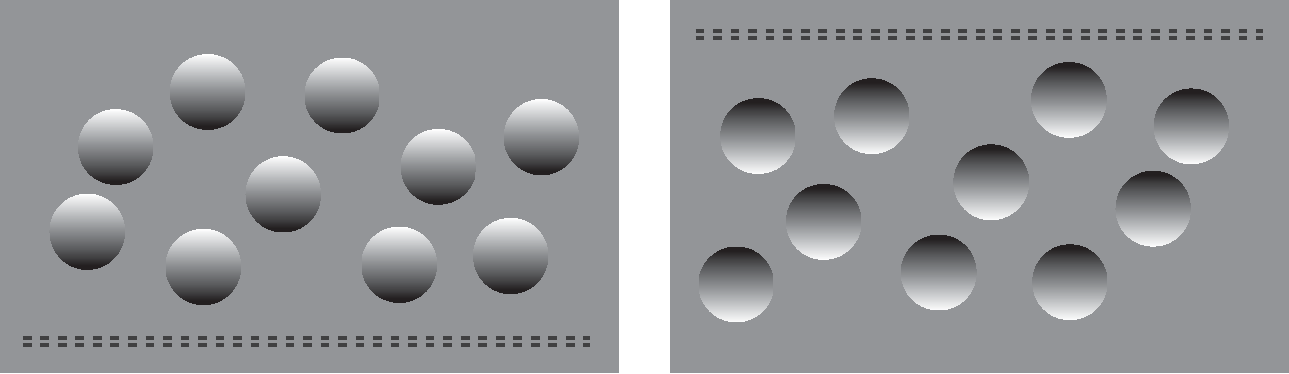
\includegraphics{resources/images/bothconcaveconvex.png}

}

\caption{concave}

\end{figure}
\end{frame}

\begin{frame}{A Brief description of a person}
\protect\hypertarget{a-brief-description-of-a-person-1}{}
\begin{itemize}
\tightlist
\item
  \textbf{Ben} - envious - stubborn - critical - impulsive - industrious
  - intelligent
\end{itemize}

\begin{itemize}
\tightlist
\item
  Keep this description in your mind(you will be asked about it later)
\end{itemize}
\end{frame}

\begin{frame}{Omission Bias}
\protect\hypertarget{omission-bias}{}
\begin{itemize}[<+->]
\item
  Bias for inaction over action (e.g., Baron \& Ritov, 2004)
\item
  Examples

  \begin{itemize}[<+->]
  \tightlist
  \item
    Financial decisions

    \begin{itemize}[<+->]
    \tightlist
    \item
      investments
    \item
      pension funds
    \end{itemize}
  \item
    Medical decisions

    \begin{itemize}[<+->]
    \tightlist
    \item
      vaccinations
    \item
      dietary medication
    \end{itemize}
  \end{itemize}
\item
  Linked to risk aversion?
\end{itemize}
\end{frame}

\begin{frame}{Description of a person}
\protect\hypertarget{description-of-a-person}{}
\url{https://app.sli.do/event/nneYhDxSeCtKayQUfCHSUQ/embed/polls/a5ba9010-98f3-41e3-a48d-57f99897aad1}

Who do you view more favourably?

Alan or Ben?
\end{frame}

\begin{frame}{Description of a person}
\protect\hypertarget{description-of-a-person-1}{}
\url{https://wall.sli.do/event/nneYhDxSeCtKayQUfCHSUQ?section=64385e8c-2f5c-481e-bbfb-6cb23b036ca8}
\end{frame}

\begin{frame}{Description of a person}
\protect\hypertarget{description-of-a-person-2}{}
Who do you view more favourably?

Alan or Ben?

\begin{itemize}
\tightlist
\item
  \textbf{Alan}:
  intelligent-industrious-impulsive-critical-stubborn-envious
\end{itemize}

\begin{itemize}
\tightlist
\item
  \textbf{Ben}:
  envious-stubborn-critical-impulsive-industrious-intelligent(Asch,
  1946; Kahneman, 2011)
\end{itemize}
\end{frame}

\begin{frame}{The Halo Effect}
\protect\hypertarget{the-halo-effect}{}
\begin{itemize}
\tightlist
\item
  ``The tendency to like (or dislike) everything about a
  person---including things you have not observed---is known as the halo
  effect''(Kahneman, 2011, p. 81)
\end{itemize}

\begin{itemize}
\tightlist
\item
  Political Leaders?
\item
  Sports people?
\item
  Artists/Actors?
\end{itemize}
\end{frame}

\begin{frame}{The Halo Effect}
\protect\hypertarget{the-halo-effect-1}{}
\href{https://www.youtube.com/embed/pWgyy_rlmag\%22\%20frameborder}{https://www.youtube.com/embed/pWgyy\_rlmag''
frameborder}
\end{frame}

\begin{frame}{Halo Effect - Moneyball}
\protect\hypertarget{halo-effect---moneyball}{}
\begin{itemize}
\tightlist
\item
  ``Good Face''
\end{itemize}

\begin{itemize}
\tightlist
\item
  ``Good Jaw''
\end{itemize}

\begin{itemize}
\tightlist
\item
  ``Can he Hit''?(Bennett, 2011)
\end{itemize}
\end{frame}

\begin{frame}{Action Bias}
\protect\hypertarget{action-bias}{}
\begin{itemize}
\item
  Bias for action over inaction (Bar-Eli, Azar, Ritov, Keidar-Levin, \&
  Schein, 2007; e.g., Patt \& Zeckhauser, 2000)
\item
  Examples

  \begin{itemize}
  \tightlist
  \item
    Government policies

    \begin{itemize}
    \tightlist
    \item
      regulating markets
    \item
      response to crises
    \end{itemize}
  \item
    Sport

    \begin{itemize}
    \tightlist
    \item
      Goal-keepers in soccer penalties
    \end{itemize}
  \end{itemize}
\item
  (Links with Social Functionalist Theory?)
\end{itemize}
\end{frame}

\begin{frame}{Wason's Rule Discovery Game}
\protect\hypertarget{wasons-rule-discovery-game}{}
(Wason, 1960)

\begin{itemize}
\item
  I will provide a sequence of 3 numbers
\item
  The sequence follows a simple rule
\item
  You must identify the rule

  \begin{itemize}
  \tightlist
  \item
    You cannot ask for the rule
  \item
    You must try guess the rule by providing your own sequence of
    numbers
  \end{itemize}
\end{itemize}

2 - 4 - 6
\end{frame}

\begin{frame}{Results}
\protect\hypertarget{results}{}
\begin{itemize}
\tightlist
\item
  Guesses attempt to confirm hypothesised rule rather than break the
  rule

  \begin{itemize}
  \tightlist
  \item
    e.g.,
  \item
    hypothesised rule: ``go up in 2s''

    \begin{itemize}
    \tightlist
    \item
      \(8 - 10 - 12\)
    \item
      \(10 - 12 - 14\)
    \end{itemize}
  \item
    hypothesised rule: ``add first two numbers to get third''

    \begin{itemize}
    \tightlist
    \item
      \(3 - 7 - 10\)
    \item
      \(4 - 9 - 13\)
    \end{itemize}
  \end{itemize}
\item
  What was the rule???
\end{itemize}
\end{frame}

\begin{frame}{Confirmation bias}
\protect\hypertarget{confirmation-bias}{}
\begin{itemize}
\tightlist
\item
  People search for evidence to confirm their beliefs rather than to
  falsify them

  \begin{itemize}
  \tightlist
  \item
    Positive testing
  \item
    Matching bias (Todd \& Gigerenzer, 2012, p. 324)
  \end{itemize}
\item
  Examples?

  \begin{itemize}
  \tightlist
  \item
    All swans are white
  \item
    ``This always happens to me!''
  \item
    Queues in a shopping centre
  \end{itemize}
\end{itemize}
\end{frame}

\begin{frame}{Syllogisms}
\protect\hypertarget{syllogisms}{}
\begin{itemize}
\tightlist
\item
  Deductive reasoning task:

  \begin{itemize}
  \tightlist
  \item
    a major premise, a minor premise, and a conclusion (Evans, 2003)
  \end{itemize}
\item
  No police dogs are vicious
\item
  Some highly trained dogs are vicious

  \begin{itemize}
  \tightlist
  \item
    Therefore, some highly trained dogs are not police dogs
  \end{itemize}
\item
  valid / invalid
\end{itemize}
\end{frame}

\begin{frame}{Syllogisms - Example 1}
\protect\hypertarget{syllogisms---example-1}{}
\begin{itemize}
\tightlist
\item
  No cigarettes are inexpensive.
\item
  Some addictive things are inexpensive.

  \begin{itemize}
  \tightlist
  \item
    Therefore, some addictive things are not cigarettes.
  \end{itemize}
\end{itemize}

Vote:
\url{https://app.sli.do/event/vZrcEo7RhhsSUSnemAjwoF/embed/polls/959fadbf-b78a-44a7-8976-7cf2f93922af}
\end{frame}

\begin{frame}{Syllogisms - Example 1}
\protect\hypertarget{syllogisms---example-1-1}{}
\url{https://wall.sli.do/event/vZrcEo7RhhsSUSnemAjwoF?section=8c85a23a-eb31-4052-97ee-49a3c76e970c}
\end{frame}

\begin{frame}{Syllogisms - Example 2}
\protect\hypertarget{syllogisms---example-2}{}
\begin{itemize}
\tightlist
\item
  No addictive things are inexpensive.
\item
  Some cigarettes are inexpensive.

  \begin{itemize}
  \tightlist
  \item
    Therefore, some addictive things are not cigarettes.
  \end{itemize}
\end{itemize}

Vote:
\url{https://app.sli.do/event/vZrcEo7RhhsSUSnemAjwoF/embed/polls/959fadbf-b78a-44a7-8976-7cf2f93922af}
\end{frame}

\begin{frame}{Syllogisms - Example 2}
\protect\hypertarget{syllogisms---example-2-1}{}
\url{https://wall.sli.do/event/vZrcEo7RhhsSUSnemAjwoF?section=8c85a23a-eb31-4052-97ee-49a3c76e970c}
\end{frame}

\begin{frame}{Syllogisms - Example 3}
\protect\hypertarget{syllogisms---example-3}{}
\begin{itemize}
\tightlist
\item
  No addictive things are inexpensive.
\item
  Some cigarettes are inexpensive.

  \begin{itemize}
  \tightlist
  \item
    Therefore, some cigarettes are not addictive.
  \end{itemize}
\end{itemize}

Vote:
\url{https://app.sli.do/event/vZrcEo7RhhsSUSnemAjwoF/embed/polls/959fadbf-b78a-44a7-8976-7cf2f93922af}
\end{frame}

\begin{frame}{Syllogisms - Example 3}
\protect\hypertarget{syllogisms---example-3-1}{}
\url{https://wall.sli.do/event/vZrcEo7RhhsSUSnemAjwoF?section=8c85a23a-eb31-4052-97ee-49a3c76e970c}
\end{frame}

\begin{frame}{Syllogisms - Example 4}
\protect\hypertarget{syllogisms---example-4}{}
\begin{itemize}
\tightlist
\item
  No cigarettes are inexpensive.
\item
  Some addictive things are inexpensive.

  \begin{itemize}
  \tightlist
  \item
    Therefore, some cigarettes are not addictive.
  \end{itemize}
\end{itemize}

Vote:
\url{https://app.sli.do/event/vZrcEo7RhhsSUSnemAjwoF/embed/polls/959fadbf-b78a-44a7-8976-7cf2f93922af}
\end{frame}

\begin{frame}{Syllogisms - Example 4}
\protect\hypertarget{syllogisms---example-4-1}{}
\url{https://wall.sli.do/event/vZrcEo7RhhsSUSnemAjwoF?section=8c85a23a-eb31-4052-97ee-49a3c76e970c}
\end{frame}

\begin{frame}{Belief Bias}
\protect\hypertarget{belief-bias}{}
\begin{longtable}[]{@{}
  >{\raggedright\arraybackslash}p{(\columnwidth - 4\tabcolsep) * \real{0.0588}}
  >{\raggedright\arraybackslash}p{(\columnwidth - 4\tabcolsep) * \real{0.4706}}
  >{\raggedright\arraybackslash}p{(\columnwidth - 4\tabcolsep) * \real{0.4706}}@{}}
\toprule\noalign{}
\begin{minipage}[b]{\linewidth}\raggedright
S.
\end{minipage} & \begin{minipage}[b]{\linewidth}\raggedright
Believable
\end{minipage} & \begin{minipage}[b]{\linewidth}\raggedright
Unbelievable
\end{minipage} \\
\midrule\noalign{}
\endhead
Valid & No cigarettes are inexpensive. Some addictive things are
inexpensive. Therefore, some addictive things are not
cigarettes.\textbf{P(``Valid'') = 92\%} & No addictive things are
inexpensive. Some cigarettes are inexpensive. Therefore, some cigarettes
are not addictive.\textbf{P(``Valid'') = 46\%} \\
Invalid & No addictive things are inexpensive. Some cigarettes are
inexpensive. Therefore, some addictive things are not cigarettes.
\textbf{P(``Valid'') = 92\%} & No cigarettes are inexpensive. Some
addictive things are inexpensive. Therefore, some cigarettes are not
addictive. \textbf{P(``Valid'') = 8\%} \\
\bottomrule\noalign{}
\end{longtable}

(Evans, Barston, \& Pollard, 1983; see also Dube, Rotello, \& Heit,
2010)
\end{frame}

\hypertarget{other-biases}{%
\section{Other Biases}\label{other-biases}}

\begin{frame}{Hindsight bias}
\protect\hypertarget{hindsight-bias}{}
\begin{itemize}
\item
  The ``I knew it all along'' effect
\item
  ``The tendency to revise the history of one's beliefs in light of what
  actually happened''(Kahneman, 2011, p. 198)
\end{itemize}
\end{frame}

\begin{frame}{Outcome bias}
\protect\hypertarget{outcome-bias}{}
\begin{itemize}
\item
  The ``You should have known'' effect
\item
  We \textbf{blame} decision makers for \emph{good decisions that worked
  out badly}

  \begin{itemize}
  \tightlist
  \item
    and give them \textbf{too little credit} for \emph{successful}
    decisions that appear obvious only after the fact
  \end{itemize}
\item
  Particularly unkind to decision makers who act as agents for others

  \begin{itemize}
  \tightlist
  \item
    physicians
  \item
    financial advisers / CEOs
  \item
    social workers
  \item
    diplomats
  \item
    politicians(Kahneman, 2011, p. 198)
  \end{itemize}
\end{itemize}
\end{frame}

\begin{frame}{General Knowledge}
\protect\hypertarget{general-knowledge}{}
\begin{itemize}
\tightlist
\item
  Which city has more inhabitants?

  \begin{itemize}
  \tightlist
  \item
    Hyderabad
  \item
    Islamabad
  \end{itemize}
\item
  How confident are you that your answer is correct?

  \begin{itemize}
  \tightlist
  \item
    50\% 60\% 70\% 80\% 90\% 100\%
  \end{itemize}
\end{itemize}

Vote:
\url{https://app.sli.do/event/2HpLUzYw48QzsHH3KWQgn7/embed/polls/adad10e1-e61e-4dce-a593-96b7e700c82e}
\end{frame}

\begin{frame}{General Knowledge}
\protect\hypertarget{general-knowledge-1}{}
\url{https://wall.sli.do/event/2HpLUzYw48QzsHH3KWQgn7?section=05f53be4-c1af-4408-a058-142bc49c3280}
\end{frame}

\begin{frame}{Overconfidence bias}
\protect\hypertarget{overconfidence-bias}{}
\begin{itemize}
\tightlist
\item
  Hyderabad

  \begin{itemize}
  \tightlist
  \item
    1,734,309
  \end{itemize}
\item
  Islamabad

  \begin{itemize}
  \tightlist
  \item
    1,009,832
  \end{itemize}
\item
  The ``systematic discrepancy between confidence judgments and the
  proportion of correct answers''(Todd \& Gigerenzer, 2012, p. 93)
\end{itemize}
\end{frame}

\begin{frame}{Biases Summary}
\protect\hypertarget{biases-summary}{}
\begin{columns}[T]
\begin{column}{0.5\textwidth}
\textbf{Covered today:}

omission bias

halo effect

action bias

confirmation bias

belief bias

hindsight bias

confidence bias

outcome bias
\end{column}

\begin{column}{0.5\textwidth}
\textbf{Other biases:}

optimistic bias

planning fallacy
\end{column}
\end{columns}
\end{frame}

\begin{frame}{Some Critiques of Biases}
\protect\hypertarget{some-critiques-of-biases}{}
\begin{itemize}
\item
  Dube et al. (2010) claim that belief bias is just a response bias
\item
  Omission bias vs Action bias?

  \begin{itemize}
  \tightlist
  \item
    bias to conform?
  \item
    bias to adhere to norms?
  \end{itemize}
\item
  Any other critiques?
\end{itemize}
\end{frame}

\begin{frame}{Activity
(\href{https://docs.google.com/document/d/1ap7xShuXe9tIzDQOky54idFdKo3teKMHsJtClSxKUGg/edit?usp=sharing}{link})}
\protect\hypertarget{activity-link}{}
\end{frame}

\hypertarget{heuristics}{%
\section{Heuristics}\label{heuristics}}

\begin{frame}{Heuristics}
\protect\hypertarget{heuristics-1}{}
\begin{itemize}
\item
  ``The term \emph{heuristic} is of Greek origin, meaning \emph{serving
  to find out or discover.}(Gigerenzer \& Todd, 1999, p. 25)
\item
  In 1905, Einstein published \emph{On a heuristic point of view
  concerning the generation and transformation of light.}

  \begin{itemize}
  \tightlist
  \item
    (Nobel prize winning paper)
  \item
    Einstein used the term \emph{heuristic} to indicate that he
    considered the view he presented as

    \begin{itemize}
    \tightlist
    \item
      incomplete
    \item
      false even
    \item
      but still useful(Gigerenzer \& Todd, 1999, p. 25)
    \end{itemize}
  \end{itemize}
\end{itemize}
\end{frame}

\begin{frame}{Heuristics}
\protect\hypertarget{heuristics-2}{}
\begin{itemize}
\tightlist
\item
  In modern psychology, the term Heuristic has come to mean a

  \begin{itemize}
  \tightlist
  \item
    \textbf{mental shortcut} or \textbf{a rule of thumb} for decision
    making,
  \item
    to help people make a quick, \textbf{satisfactory}
  \item
    \textbf{but perhaps not perfect} answer to a complex question
  \end{itemize}
\item
  ``A heuristic is any \emph{rule of thumb} or simple rule of behavior
  by which a person solves a problem'' (Cartwright, 2014, p. 33)

  \begin{itemize}
  \tightlist
  \item
    e.g., the shopper can solve their problem of what cereal to buy with
    the heuristic, `buy what I usually do'(Cartwright, 2014, p. 33)
  \end{itemize}
\item
  Domain specific (Gigerenzer \& Selten, 2002, pp. 7, 41)
\end{itemize}
\end{frame}

\begin{frame}{Catching a ball}
\protect\hypertarget{catching-a-ball}{}
\begin{itemize}
\item
  How does an outfielder catch a ball?

  \begin{itemize}
  \tightlist
  \item
    H1: Computing the balls trajectory?
  \item
    H2: Gaze Heuristic
  \end{itemize}
\item
  H1: Trajectory computation predicts that players first estimate the
  point where the ball will come down, then run as fast as they can to
  this point and wait for the ball. (Todd \& Gigerenzer, 2012, p. 28)
\item
  H2: Gaze Heuristic predicts that players fix their gaze on the ball,
  start running, and adjust running speed so that the angle of gaze
  remains constant.

  \begin{itemize}
  \tightlist
  \item
    predicts changes in speed
  \item
    predicts slight arc in certain situations
  \end{itemize}
\end{itemize}
\end{frame}

\begin{frame}{Computing the Trajectory}
\protect\hypertarget{computing-the-trajectory}{}
\begin{figure}

{\centering 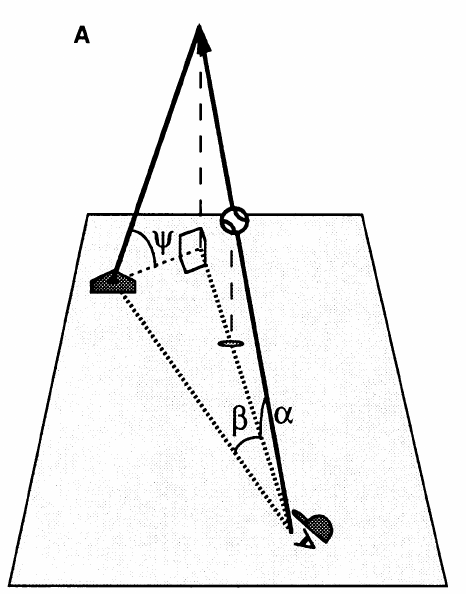
\includegraphics{resources/images/gaze_calculation.png}

}

\caption{calculation}

\end{figure}

\(\tan{\Psi} = \frac{\tan{\alpha}}{\tan{\beta}} = \frac{C_\alpha f(t)}{C_\beta f(t)} = C_\Psi\)

\begin{itemize}
\tightlist
\item
  where \(C_\alpha\), \(C_\beta\) and \(C_\Psi\) are constants and
  \(f(t) = t =\) time since trajectory (taken from McBeath, Shaffer, \&
  Kaiser, 1995, p. 571)
\end{itemize}
\end{frame}

\begin{frame}{Gaze Heuristic}
\protect\hypertarget{gaze-heuristic}{}
\begin{figure}

{\centering 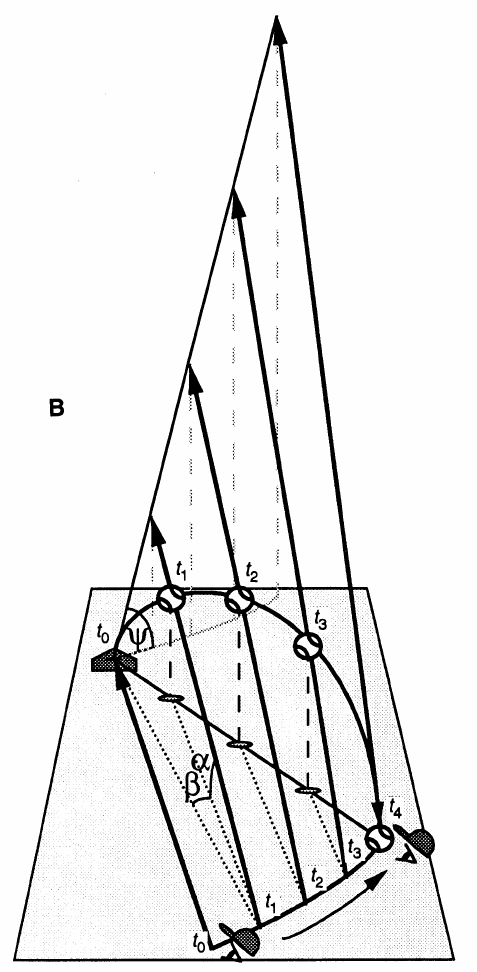
\includegraphics{resources/images/McBeath.png}

}

\caption{gaze}

\end{figure}

(taken from McBeath et al., 1995, p. 571)
\end{frame}

\begin{frame}{Catching a ball}
\protect\hypertarget{catching-a-ball-1}{}
\begin{figure}

{\centering 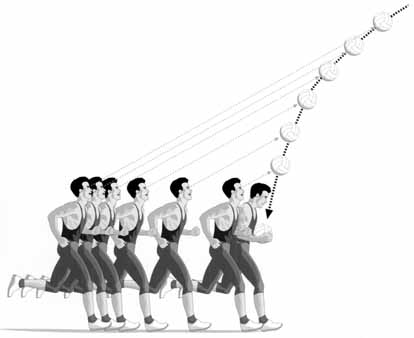
\includegraphics{resources/images/gaze.jpg}

}

\caption{gaze}

\end{figure}
\end{frame}

\begin{frame}{Gaze Heuristic}
\protect\hypertarget{gaze-heuristic-1}{}
\url{https://www.youtube.com/embed/-J1qryj6kdg}
\end{frame}

\begin{frame}{Catching a ball}
\protect\hypertarget{catching-a-ball-2}{}
\begin{itemize}
\tightlist
\item
  H2: Gaze Heuristic predicts that players fix their gaze on the ball,
  start running, and adjust running speed so that the angle of gaze
  remains constant.
\item
  predicts changes in speed
\item
  predicts slight arc in certain situations

  \begin{itemize}
  \tightlist
  \item
    \textbf{All Observed}
  \end{itemize}
\end{itemize}
\end{frame}

\begin{frame}{3D Heuristic}
\protect\hypertarget{d-heuristic}{}
\begin{figure}

{\centering 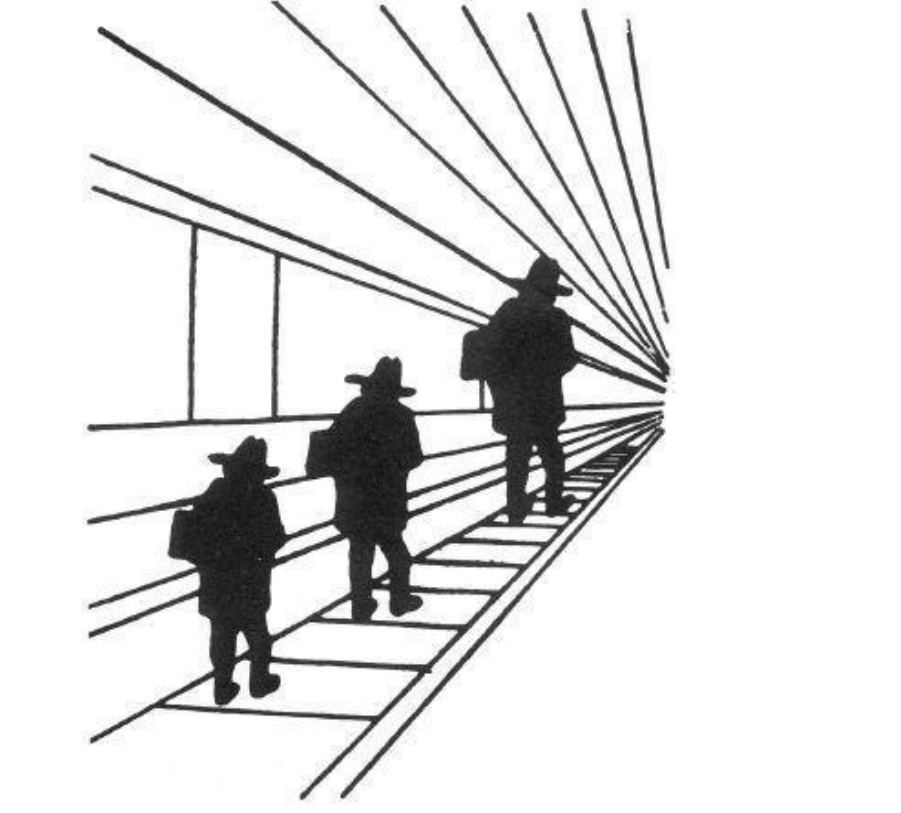
\includegraphics{resources/images/3dheuristic.png}

}

\caption{3d}

\end{figure}
\end{frame}

\hypertarget{more-general-heuristics}{%
\section{More General Heuristics}\label{more-general-heuristics}}

\begin{frame}{Word task}
\protect\hypertarget{word-task}{}
\begin{itemize}
\tightlist
\item
  Consider the letter K.
\end{itemize}

\begin{itemize}
\tightlist
\item
  Is K more likely to appear as the first letter in a word OR as the
  third letter?
\end{itemize}
\end{frame}

\begin{frame}{Word task}
\protect\hypertarget{word-task-1}{}
\begin{itemize}
\tightlist
\item
  Consider the letter L.
\end{itemize}

\begin{itemize}
\tightlist
\item
  Is L more likely to appear as the first letter in a word OR as the
  third letter?
\end{itemize}
\end{frame}

\begin{frame}{Word task}
\protect\hypertarget{word-task-2}{}
\begin{itemize}
\item
  Also true for the letters N, R, V
\item
  How did you do it?
\item
  It is easier to come up with words using the first letter than the
  third letter
\item
  More \textbf{available} examples
\end{itemize}
\end{frame}

\begin{frame}{The Availability Heuristic}
\protect\hypertarget{the-availability-heuristic}{}
\begin{itemize}
\tightlist
\item
  the process of judging frequency by ``the ease with which instances
  come to mind''(Kahneman, 2011, p. 128)
\end{itemize}

\begin{itemize}
\tightlist
\item
  e.g., think of the number of words that can be constructed from the
  two sets of letters below.

  \begin{itemize}
  \tightlist
  \item
    XUZONLCJM
  \item
    TAPCERHOB
  \end{itemize}
\end{itemize}
\end{frame}

\begin{frame}{The Availability Heuristic}
\protect\hypertarget{the-availability-heuristic-1}{}
\begin{itemize}
\tightlist
\item
  Inflated Salience

  \begin{itemize}
  \tightlist
  \item
    e.g., high media coverage of:

    \begin{itemize}
    \tightlist
    \item
      Divorces among Hollywood celebrities
    \item
      Sex scandals among politicians
    \end{itemize}
  \item
    people exaggerate the frequency of both
  \end{itemize}
\item
  Dramatic events

  \begin{itemize}
  \tightlist
  \item
    A plane crash that attracts media coverage will temporarily alter
    your feelings about the safety of flying
  \item
    after you see a car burning at the side of the road, accidents are
    on your mind and the world is for a while a more dangerous place.
  \end{itemize}
\end{itemize}
\end{frame}

\begin{frame}{The Availability Heuristic}
\protect\hypertarget{the-availability-heuristic-2}{}
\begin{itemize}
\tightlist
\item
  Personal experiences, pictures, vivid examples

  \begin{itemize}
  \tightlist
  \item
    \textbf{more available} than incidents that happen to others, mere
    words, or statistics
  \item
    e.g., a judicial error that affects you will undermine your faith in
    the justice system more than a similar incident that you read
    about(Kahneman, 2011, p. 129)
  \end{itemize}
\end{itemize}
\end{frame}

\begin{frame}{Practical Examples}
\protect\hypertarget{practical-examples}{}
\begin{itemize}
\tightlist
\item
  Ross \& Sicoly (1979) housework study
\end{itemize}

\begin{itemize}
\tightlist
\item
  First, list six instances in which you behaved assertively

  \begin{itemize}
  \tightlist
  \item
    Evaluate how assertive you are
  \end{itemize}
\item
  Now list 12 instances in which you behaved assertively

  \begin{itemize}
  \tightlist
  \item
    Evaluate how assertive you are(Schwarz, Bless, Strack, Klumpp, \& et
    al, 1991)
  \end{itemize}
\end{itemize}
\end{frame}

\begin{frame}{Practical Examples (continued)}
\protect\hypertarget{practical-examples-continued}{}
\begin{itemize}
\tightlist
\item
  It has been found that people:

  \begin{itemize}
  \tightlist
  \item
    believe that they use their bicycles less often after recalling many
    rather than few instances
  \item
    are less confident in a choice when they are asked to produce more
    arguments to support it
  \item
    are less confident that an event was avoidable after listing more
    ways it could have been avoided
  \item
    are less impressed by a car after listing many of its
    advantages(Kahneman, 2011)
  \end{itemize}
\end{itemize}
\end{frame}

\begin{frame}{Heuristics and Errors}
\protect\hypertarget{heuristics-and-errors}{}
\begin{itemize}
\tightlist
\item
  A psychologist wrote thumbnail descriptions of a sample of 1000
  participants consisting of 995 females and 5 males. The description
  below was chosen at random from the 1,000 available descriptions.
\end{itemize}

\begin{itemize}
\tightlist
\item
  Jo is 23 years old and is finishing a degree in engineering. On Friday
  nights, Jo likes to go out cruising with friends while listening to
  loud music and drinking beer.
\end{itemize}

\begin{itemize}
\tightlist
\item
  Which one of the following two statements is most likely?

  \begin{itemize}
  \tightlist
  \item
    Jo is a man
  \item
    Jo is a woman
  \end{itemize}
\end{itemize}
\end{frame}

\begin{frame}{Representativeness Heuristic}
\protect\hypertarget{representativeness-heuristic}{}
\begin{itemize}
\tightlist
\item
  judging a situation based on how similar the prospects are to the
  prototypes the person holds in his or her mind.
\end{itemize}
\end{frame}

\begin{frame}{Representativeness Heuristic}
\protect\hypertarget{representativeness-heuristic-1}{}
\begin{itemize}
\tightlist
\item
  Linda is thirty-one years old, single, outspoken, and very bright. She
  majored in philosophy. As a student, she was deeply concerned with
  issues of discrimination and social justice, and also participated in
  antinuclear demonstrations.
\end{itemize}

\begin{itemize}
\tightlist
\item
  Which alternative is more probable?

  \begin{itemize}
  \tightlist
  \item
    Linda is a bank teller.
  \item
    Linda is a bank teller and is active in the feminist movement.
  \end{itemize}
\item
  Conjunction fallacy

  \begin{itemize}
  \tightlist
  \item
    (and belief bias?)
  \end{itemize}
\end{itemize}
\end{frame}

\begin{frame}{Anchoring}
\protect\hypertarget{anchoring}{}
\begin{itemize}
\item
  Taking information salient in the environment and using it to
  \emph{anchor} your decisions
\item
  e.g., rigged wheel of fortune: 10 or 65

  \begin{itemize}
  \tightlist
  \item
    Is the percentage of African nations among UN members larger or
    smaller than the number you just wrote?
  \item
    What is your best guess of the percentage of African nations in the
    UN?
  \end{itemize}
\item
  Mean response 25\% and 45\% (depending on 10 or 65)
\end{itemize}
\end{frame}

\begin{frame}{Mood Heuristic}
\protect\hypertarget{mood-heuristic}{}
\begin{itemize}
\item
  How happy are you these days?
\item
  How many dates did you have last month?
\item
  correlation?
\end{itemize}
\end{frame}

\begin{frame}{Mood Heuristic}
\protect\hypertarget{mood-heuristic-1}{}
\begin{itemize}
\tightlist
\item
  How many dates did you have last month?
\item
  How happy are you these days?
\end{itemize}
\end{frame}

\begin{frame}{The Affect Heuristic}
\protect\hypertarget{the-affect-heuristic}{}
\begin{itemize}
\item
  ``people let their likes and dislikes determine their beliefs about
  the world''(Kahneman, 2011, p. 102)
\item
  Substitution

  \begin{itemize}
  \tightlist
  \item
    How do I feel about it?
  \end{itemize}
\item
  serves as an answer to a much harder question

  \begin{itemize}
  \tightlist
  \item
    What do I think about it? (Kahneman, 2011; Slovic, Peters, Finucane,
    \& MacGregor, 2005)
  \end{itemize}
\end{itemize}
\end{frame}

\begin{frame}{Other Heuristics}
\protect\hypertarget{other-heuristics}{}
\begin{figure}

{\centering 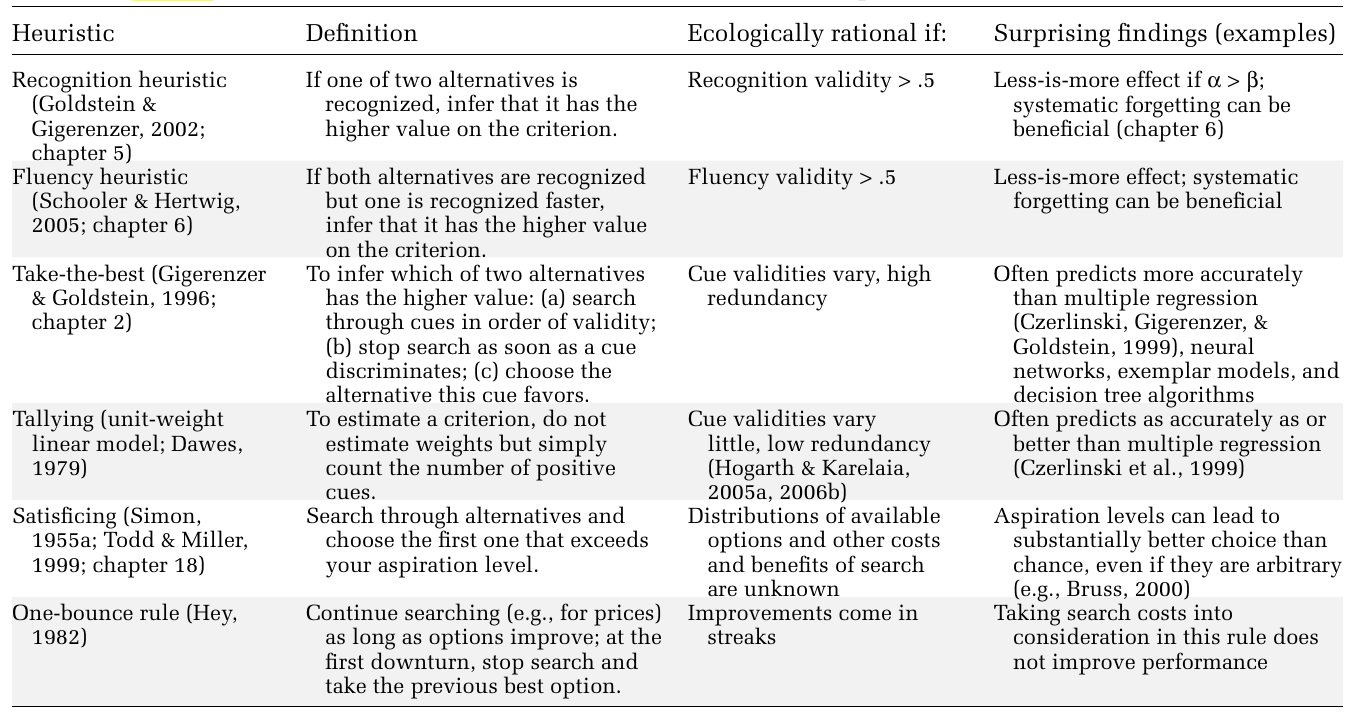
\includegraphics{resources/images/heuristics_table1.png}

}

\caption{table}

\end{figure}

(taken from Todd \& Gigerenzer, 2012, p. 9)
\end{frame}

\begin{frame}{Other Heuristics}
\protect\hypertarget{other-heuristics-1}{}
\begin{figure}

{\centering 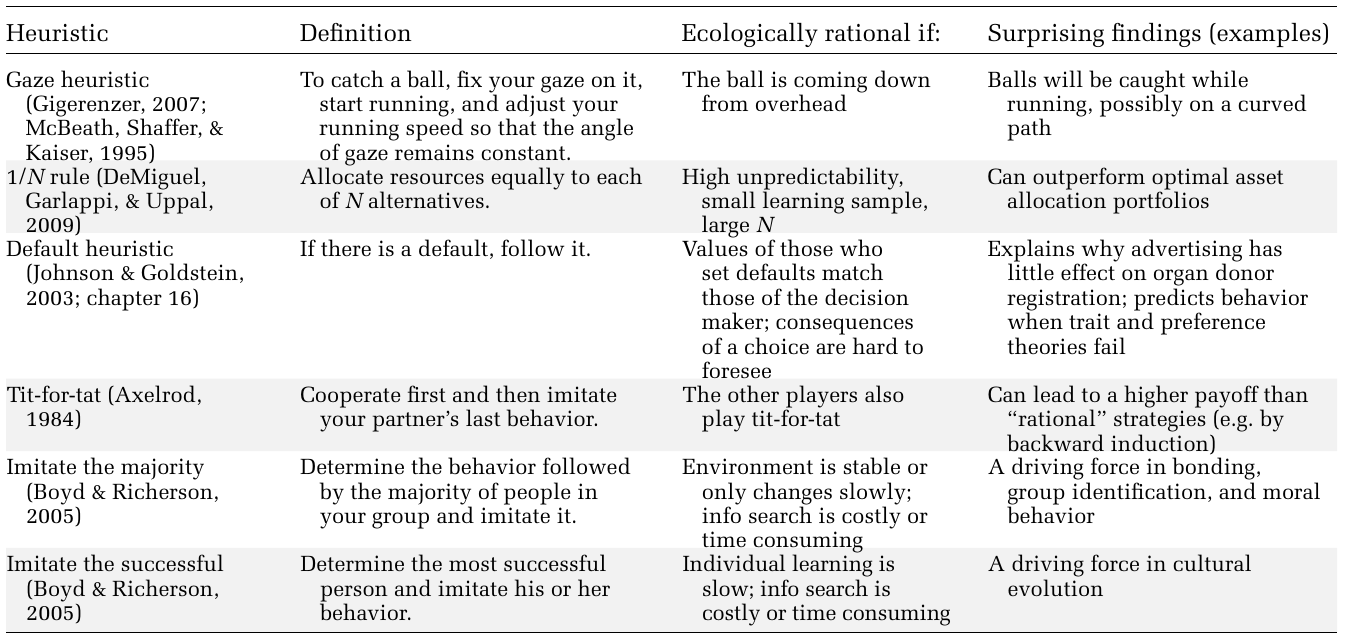
\includegraphics{resources/images/heuristics_table2.png}

}

\caption{table}

\end{figure}

(taken from Todd \& Gigerenzer, 2012, p. 10)
\end{frame}

\hypertarget{in-class-activity}{%
\section{In-Class Activity}\label{in-class-activity}}

\begin{frame}{In-Class Activity}
\protect\hypertarget{in-class-activity-1}{}
\begin{itemize}
\tightlist
\item
  In groups:

  \begin{itemize}
  \tightlist
  \item
    Identify possible \emph{novel} heuristics
  \end{itemize}
\end{itemize}

\pause

Possible Examples:

\begin{itemize}
\item
  Watching sport

  \begin{itemize}
  \tightlist
  \item
    Camera gaze heuristic
  \item
    Waving flags heuristic
  \end{itemize}
\item
  Music

  \begin{itemize}
  \tightlist
  \item
    Chord-notes heuristic
  \end{itemize}
\item
  Copy others heuristic (novel situations/uncertainty)
\item
  Empty seats on a bus/in class?
\item
  Choosing a till in the supermarket?
\end{itemize}
\end{frame}

\begin{frame}{Activity:(\href{https://docs.google.com/document/d/1ap7xShuXe9tIzDQOky54idFdKo3teKMHsJtClSxKUGg/edit?usp=sharing}{link})}
\protect\hypertarget{activitylink}{}
\url{https://docs.google.com/document/d/1ap7xShuXe9tIzDQOky54idFdKo3teKMHsJtClSxKUGg/edit?embedded=true\&rm=minimal}
\end{frame}

\hypertarget{references}{%
\section{References}\label{references}}

\begin{frame}{References}
\protect\hypertarget{references-1}{}
\end{frame}

\begin{frame}{References}
\protect\hypertarget{references-2}{}
\noindent \vspace{-2em} \setlength{\parindent}{-0.5in}
\setlength{\leftskip}{0.5in} \setlength{\parskip}{7.5pt}

\hypertarget{refs}{}
\begin{CSLReferences}{1}{0}
\leavevmode\vadjust pre{\hypertarget{ref-asch_forming_1946}{}}%
Asch, S. E. (1946). Forming impressions of personality. \emph{The
Journal of Abnormal and Social Psychology}, \emph{41}(3), 258.

\leavevmode\vadjust pre{\hypertarget{ref-bar-eli_action_2007}{}}%
Bar-Eli, M., Azar, O. H., Ritov, I., Keidar-Levin, Y., \& Schein, G.
(2007). Action bias among elite soccer goalkeepers: {The} case of
penalty kicks. \emph{Journal of Economic Psychology}, \emph{28}(5),
606--621. \url{https://doi.org/10.1016/j.joep.2006.12.001}

\leavevmode\vadjust pre{\hypertarget{ref-baron_omission_2004}{}}%
Baron, J., \& Ritov, I. (2004). Omission bias, individual differences,
and normality. \emph{Organizational Behavior and Human Decision
Processes}, \emph{94}(2), 74--85.
\url{https://doi.org/10.1016/j.obhdp.2004.03.003}

\leavevmode\vadjust pre{\hypertarget{ref-bennett_moneyball_2011}{}}%
Bennett, M. (2011). Moneyball.

\leavevmode\vadjust pre{\hypertarget{ref-cartwright_behavioral_2014}{}}%
Cartwright, E. (2014). \emph{Behavioral economics}. {New York}:
{Routledge}.

\leavevmode\vadjust pre{\hypertarget{ref-dube_assessing_2010}{}}%
Dube, C., Rotello, C. M., \& Heit, E. (2010). Assessing the {Belief Bias
Effect With Rocs}: {It}'s a {Response Bias Effect}. \emph{Psychological
Review}, \emph{117}(3), 831--863. \url{https://doi.org/10.1037/a0019634}

\leavevmode\vadjust pre{\hypertarget{ref-evans_two_2003}{}}%
Evans, J. St. B. T. (2003). In two minds: Dual-process accounts of
reasoning. \emph{Trends in Cognitive Sciences}, \emph{7}(10), 454--459.
\url{https://doi.org/10.1016/j.tics.2003.08.012}

\leavevmode\vadjust pre{\hypertarget{ref-evans_conflict_1983}{}}%
Evans, J. St. B. T., Barston, J. L., \& Pollard, P. (1983). On the
conflict between logic and belief in syllogistic reasoning. \emph{Memory
\& Cognition}, \emph{11}(3), 295--306.
\url{https://doi.org/10.3758/BF03196976}

\leavevmode\vadjust pre{\hypertarget{ref-eysenck_cognitive_2005}{}}%
Eysenck, M. W., \& Keane, M. T. (2005). \emph{Cognitive psychology: A
student's handbook}. {Hove {[}England{]}; New York}: {Psychology Press}.

\leavevmode\vadjust pre{\hypertarget{ref-gigerenzer_bounded_2002}{}}%
Gigerenzer, G., \& Selten, R. (2002). \emph{Bounded {Rationality}: {The
Adaptive Toolbox}}. {MIT Press}.

\leavevmode\vadjust pre{\hypertarget{ref-gigerenzer_simple_1999}{}}%
Gigerenzer, G., \& Todd, P. M. (1999). \emph{Simple heuristics that make
us smart}. {New York}: {Oxford University Press}.

\leavevmode\vadjust pre{\hypertarget{ref-howe_perceiving_2005}{}}%
Howe, C. Q., \& Purves, D. (2005). \emph{Perceiving {Geometry}:
{Geometrical Illusions Explained} by {Natural Scene Statistics}}.
{Springer Science \& Business Media}.

\leavevmode\vadjust pre{\hypertarget{ref-kahneman_thinking_2011}{}}%
Kahneman, D. (2011). \emph{Thinking, fast and slow}. {London}: {Allen
Lane}.

\leavevmode\vadjust pre{\hypertarget{ref-mcbeath_how_1995}{}}%
McBeath, M. K., Shaffer, D. M., \& Kaiser, M. K. (1995). How baseball
outfielders determine where to run to catch fly balls. \emph{Science},
\emph{268}(5210), 569--573.
\url{https://doi.org/10.1126/science.7725104}

\leavevmode\vadjust pre{\hypertarget{ref-over_rationality_2004}{}}%
Over, D. E. (2004). Rationality and the {Normative}/{Descriptive
Distinction}. In N. Harvey \& D. J. Koehler (Eds.), \emph{Blackwell
handbook of judgment and decision making} (1st ed., pp. 3--18).
{Malden}: {Blackwell}.

\leavevmode\vadjust pre{\hypertarget{ref-patt_action_2000}{}}%
Patt, A., \& Zeckhauser, R. (2000). Action {Bias} and {Environmental
Decisions}. \emph{Journal of Risk and Uncertainty}, \emph{21}(1),
45--72. \url{https://doi.org/10.1023/A:1026517309871}

\leavevmode\vadjust pre{\hypertarget{ref-reber_penguin_2001}{}}%
Reber, A. S. (2001). \emph{The {Penguin} dictionary of psychology} (3rd
ed). {London ; New York}: {Penguin Books}.

\leavevmode\vadjust pre{\hypertarget{ref-ross_egocentric_1979}{}}%
Ross, M., \& Sicoly, F. (1979). Egocentric biases in availability and
attribution. \emph{Journal of Personality and Social Psychology},
\emph{37}(3), 322--336. \url{https://doi.org/10.1037/0022-3514.37.3.322}

\leavevmode\vadjust pre{\hypertarget{ref-schwarz_ease_1991}{}}%
Schwarz, N., Bless, H., Strack, F., Klumpp, G., \& et al. (1991). Ease
of retrieval as information: {Another} look at the availability
heuristic. \emph{Journal of Personality and Social Psychology},
\emph{61}(2), 195--202.
\url{https://doi.org/10.1037//0022-3514.61.2.195}

\leavevmode\vadjust pre{\hypertarget{ref-slovic_affect_2005}{}}%
Slovic, P., Peters, E., Finucane, M. L., \& MacGregor, D. G. (2005).
Affect, risk, and decision making. \emph{Health Psychology},
\emph{24}(4, Suppl), S35--S40.
\url{https://doi.org/10.1037/0278-6133.24.4.S35}

\leavevmode\vadjust pre{\hypertarget{ref-todd_ecological_2012}{}}%
Todd, P. M., \& Gigerenzer, G. (Eds.). (2012). \emph{Ecological
rationality: Intelligence in the world}. {Oxford ; New York}: {Oxford
University Press}.

\leavevmode\vadjust pre{\hypertarget{ref-wason_failure_1960}{}}%
Wason, P. C. (1960). On the {Failure} to {Eliminate Hypotheses} in a
{Conceptual Task}. \emph{Quarterly Journal of Experimental Psychology},
\emph{12}(3), 129--140. \url{https://doi.org/10.1080/17470216008416717}

\end{CSLReferences}
\end{frame}



\end{document}
